\documentclass[aspectratio=169, 11pt]{beamer}

% ============================================================
% THEME AND STYLING (matched to slides_example.tex)
% ============================================================
\usetheme{metropolis}
\usepackage{appendixnumberbeamer}

% Colors - Dark theme with accent colors
\definecolor{darkbg}{HTML}{1a1a2e}
\definecolor{darkfg}{HTML}{16213e}
\definecolor{accent}{HTML}{e94560}
\definecolor{accentblue}{HTML}{00d9ff}
\definecolor{textlight}{HTML}{eaeaea}
\definecolor{textsub}{HTML}{a0a0a0}

\setbeamercolor{normal text}{fg=textlight, bg=darkbg}
\setbeamercolor{alerted text}{fg=accent}
\setbeamercolor{example text}{fg=accentblue}
\setbeamercolor{frametitle}{fg=textlight, bg=darkfg}
\setbeamercolor{title}{fg=textlight}
\setbeamercolor{subtitle}{fg=textsub}
\setbeamercolor{author}{fg=textsub}
\setbeamercolor{date}{fg=textsub}
\setbeamercolor{block title}{fg=textlight, bg=darkfg}
\setbeamercolor{block body}{fg=textlight, bg=darkfg!50!darkbg}
\setbeamercolor{item}{fg=accent}
\setbeamercolor{subitem}{fg=accentblue}

% Progress bar
\metroset{progressbar=frametitle}
\setbeamercolor{progress bar}{fg=accent, bg=darkfg}

% ============================================================
% PACKAGES
% ============================================================
\usepackage{amsmath, amssymb}
\usepackage{graphicx}
\usepackage{booktabs}
\usepackage{tikz}
\usetikzlibrary{positioning, arrows.meta, shapes.geometric, fit, backgrounds}
\usepackage{xcolor}
\graphicspath{{../images/}}

% Section page styling: keep the metropolis section transitions visible
\setbeamercolor{section title}{fg=textlight}
\setbeamercolor{section in head/foot}{fg=textsub, bg=darkbg}

% Reusable TikZ styles
\tikzset{
  pipenode/.style={
    draw=accentblue, fill=darkfg, text=textlight,
    rounded corners=4pt, minimum height=1.0cm, minimum width=1.9cm,
    align=center, font=\small\bfseries, line width=0.6pt
  },
  pipearrow/.style={-{Stealth[length=2.5mm]}, line width=0.7pt, draw=accent},
  herostat/.style={
    draw=accentblue, fill=darkfg, text=textlight,
    rounded corners=6pt, minimum height=2.4cm, minimum width=4.0cm,
    align=center, line width=0.7pt
  },
  prioritybox/.style={
    draw=accent, fill=darkfg, text=textlight,
    rounded corners=3pt, minimum height=0.7cm, minimum width=2.6cm,
    align=center, font=\small, line width=0.5pt
  }
}

% ============================================================
% TITLE INFO
% ============================================================
\title{Structural Patterns in News Headlines}
\subtitle{Recovering form, framing, and rhetorical mode with interpretable rules}
\author{Victor Derani \and Avi Herman \and Kylie Lin}
\date{NLP Final Project}
\institute{Department of Computer Science}

% ============================================================
% DOCUMENT
% ============================================================
\begin{document}

% ----------------------------------------------------------
% TITLE
% ----------------------------------------------------------
\begin{frame}[plain]
  \maketitle
\end{frame}

\section{Setup}

% ----------------------------------------------------------
% QUESTION
% ----------------------------------------------------------
\begin{frame}{The Question}
  \begin{center}
    \Large
    \textcolor{accent}{Do news headlines follow stable syntactic templates}\\[0.5em]
    \textcolor{accentblue}{that can be modeled and evaluated rigorously?}\\[1.5em]
    \normalsize
    \textcolor{textsub}{Focus: linguistic form, not topic semantics.}\\[0.5em]
    \textcolor{textsub}{Goal: interpretable structure + style prediction.}
  \end{center}
\end{frame}

% ----------------------------------------------------------
% MOTIVATION
% ----------------------------------------------------------
\begin{frame}{Why Headlines?}
  \begin{columns}
    \column{0.52\textwidth}
    \textbf{Headlines are extreme compression:}
    \begin{itemize}
      \item Minimal length, maximal information
      \item Strong editorial constraints
      \item High public exposure and downstream impact
    \end{itemize}

    \vspace{0.8em}
    \textbf{NLP relevance:}
    \begin{itemize}
      \item Concise generation
      \item Summarization quality control
      \item Framing and agency analysis
    \end{itemize}

    \column{0.48\textwidth}
    \begin{block}{Core Thesis}
      Headline writing is not free-form text production; it is a constrained system with reproducible structural regularities.
    \end{block}
  \end{columns}
\end{frame}

% ----------------------------------------------------------
% HYPOTHESIS
% ----------------------------------------------------------
\begin{frame}{Hypothesis and Falsification}
  \begin{block}{Hypothesis}
    News headlines follow stable, reusable syntactic templates that are recoverable from parse-level features at rates above trivial baselines.
  \end{block}

  \vspace{0.8em}

  \textbf{Falsification criteria:}
  \begin{itemize}
    \item Macro F1 collapses toward majority/random behavior
    \item No dominant recurring templates in corpus-level analysis
    \item Large instability across random train/dev/test splits
    \item Rules cannot be linked to parse evidence
  \end{itemize}
\end{frame}

\section{Method}

% ----------------------------------------------------------
% PIPELINE
% ----------------------------------------------------------
\begin{frame}{Pipeline Overview}
  \begin{center}
    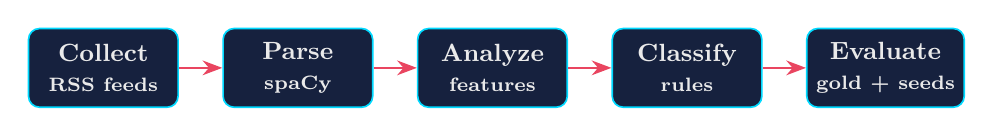
\begin{tikzpicture}[node distance=0.55cm and 0.55cm]
      \node[pipenode] (collect)  {Collect\\\scriptsize RSS feeds};
      \node[pipenode, right=of collect] (parse) {Parse\\\scriptsize spaCy};
      \node[pipenode, right=of parse]   (analyze) {Analyze\\\scriptsize features};
      \node[pipenode, right=of analyze] (classify) {Classify\\\scriptsize rules};
      \node[pipenode, right=of classify] (eval) {Evaluate\\\scriptsize gold + seeds};

      \draw[pipearrow] (collect)  -- (parse);
      \draw[pipearrow] (parse)    -- (analyze);
      \draw[pipearrow] (analyze)  -- (classify);
      \draw[pipearrow] (classify) -- (eval);
    \end{tikzpicture}
  \end{center}

  \vspace{0.3em}
  \begin{columns}
    \column{0.5\textwidth}
    \textbf{What flows through}
    \begin{itemize}
      \item Tokens, POS tags, dependencies, entities
      \item Macro POS templates and openings
      \item Rule-priority structural label
      \item Multi-dimensional style profile
    \end{itemize}

    \column{0.5\textwidth}
    \begin{block}{Parsing robustness}
      Model preference hierarchy plus normalization and a fallback parse pass for difficult casing and formatting conditions.
    \end{block}
  \end{columns}
\end{frame}

% ----------------------------------------------------------
% GOLD EXPLANATION
% ----------------------------------------------------------
\begin{frame}{What ``Gold'' Means and Why We Need It}
  \textbf{Gold-standard labels = human-verified ground truth}

  \vspace{0.8em}

  \begin{columns}
    \column{0.5\textwidth}
    \textbf{Why necessary:}
    \begin{itemize}
      \item Prevent circular evaluation
      \item Measure true error, not self-agreement
      \item Enable valid precision/recall/F1
      \item Support fair model comparisons
    \end{itemize}

    \column{0.5\textwidth}
    \textbf{Dataset design:}
    \begin{itemize}
      \item 464 manually labeled headlines
      \item Train / Dev / Test $=$ 276 / 90 / 98
      \item About 60 / 20 / 20 split, balanced for:
      \begin{itemize}
        \item rule learning capacity (train),
        \item tuning diagnostics (dev),
        \item unbiased final estimate (test)
      \end{itemize}
    \end{itemize}
  \end{columns}

  \vspace{0.8em}

  \textcolor{accent}{Without gold annotation, high scores can be meaningless.}
\end{frame}

% ----------------------------------------------------------
% MANUAL TAGGING EXAMPLES
% ----------------------------------------------------------
\begin{frame}{Manual Tagging Examples}
  \textbf{Example 1}
  \begin{itemize}
    \item Headline: \textit{Nine killed in second Turkish school shooting in two days}
    \item Gold label: \texttt{passive\_clause}
    \item Gold rhetorical mode: \texttt{straight\_report}
    \item Why: compressed passive event framing (\texttt{NUM + VBN}), omitted agent
  \end{itemize}

  \vspace{0.5em}
  \textbf{Example 2}
  \begin{itemize}
    \item Headline: \textit{Iran Update Special Report, April 14, 2026 Institute for the Study of War}
    \item Gold label: \texttt{noun\_phrase\_fragment}
    \item Gold rhetorical mode: \texttt{analysis\_explainer}
    \item Why: report-style nominal title with no finite main clause
  \end{itemize}
\end{frame}

% ----------------------------------------------------------
% WHY THESE METRICS
% ----------------------------------------------------------
\begin{frame}{Why These Metrics in This Study}
  \begin{columns}
    \column{0.52\textwidth}
    \textbf{Accuracy}
    \begin{itemize}
      \item Fraction of headlines whose predicted label equals the gold label
      \item Useful for top-line editorial reliability
    \end{itemize}

    \textbf{Precision$_c$ / Recall$_c$}
    \begin{itemize}
      \item Precision$_c$: when we predict class $c$, how often are we right?
      \item Recall$_c$: of true class-$c$ headlines, how many do we recover?
    \end{itemize}

    \column{0.48\textwidth}
    \textbf{$F1_c$}
    \begin{itemize}
      \item Harmonic mean of precision and recall for class $c$
      \item Punishes one-sided behavior
    \end{itemize}

    \textbf{Macro F1}
    \begin{itemize}
      \item Equal average over classes
      \item Critical under imbalance (`simple\_clause` dominates)
      \item Prevents "high accuracy, poor minority labels"
    \end{itemize}
  \end{columns}
\end{frame}

% ----------------------------------------------------------
% LABEL SET
% ----------------------------------------------------------
\begin{frame}{Structural and Style Label Space}
  \begin{columns}
    \column{0.52\textwidth}
    \textbf{Structure labels}
    \begin{itemize}
      \item question\_form
      \item passive\_clause
      \item coordination
      \item noun\_phrase\_fragment
      \item simple\_clause
      \item other
    \end{itemize}

    \column{0.48\textwidth}
    \textbf{Style dimensions}
    \begin{itemize}
      \item lead\_frame
      \item agency\_style
      \item density\_band
      \item rhetorical\_mode
    \end{itemize}
  \end{columns}

  \vspace{0.8em}

  \[
  \text{signature} = \text{structure}\;|\;\text{lead\_frame}\;|\;\text{rhetorical\_mode}
  \]
\end{frame}

% ----------------------------------------------------------
% METRICS
% ----------------------------------------------------------
\begin{frame}{Evaluation Metrics}
  \begin{columns}
    \column{0.56\textwidth}
    \[
    \text{Accuracy} = \frac{\#\text{correct}}{\#\text{total}}
    \]
    \[
    \text{Precision}_c = \frac{TP_c}{TP_c + FP_c},\quad
    \text{Recall}_c = \frac{TP_c}{TP_c + FN_c}
    \]
    \[
    F1_c = \frac{2PR}{P+R},\quad
    \text{Macro F1} = \frac{1}{|C|}\sum_{c\in C} F1_c
    \]

    \column{0.44\textwidth}
    \textbf{Why Macro F1 matters}
    \begin{itemize}
      \item Class imbalance is substantial
      \item Prevents dominant classes from hiding failures
      \item Better reflects minority-class behavior
    \end{itemize}

    \vspace{0.6em}
    \textbf{In our context}
    \begin{itemize}
      \item Accuracy = top-line headline match rate
      \item Macro F1 = class-balanced structural reliability
    \end{itemize}
  \end{columns}
\end{frame}

% ----------------------------------------------------------
% WORKED DECISION PATHS
% ----------------------------------------------------------
\begin{frame}{Worked Decision Paths (Classifier Logic)}
  \textbf{Question-form example}
  \begin{itemize}
    \item \textit{Are we witnessing the death of expertise?}
    \item Path: contains ``?'' $\rightarrow$ interrogative rule fires first
    \item Output: \texttt{question\_form}, \texttt{question\_hook}
  \end{itemize}

  \vspace{0.6em}
  \textbf{Passive compressed-event example}
  \begin{itemize}
    \item \textit{Nine killed in second Turkish school shooting in two days}
    \item Path: non-question $\rightarrow$ \texttt{NUM + VBN} passive cue
    \item Output: \texttt{passive\_clause}, \texttt{passive\_agent\_omitted}
  \end{itemize}
\end{frame}

\begin{frame}{Worked Decision Paths (continued)}
  \textbf{Nominal report-title example}
  \begin{itemize}
    \item \textit{Iran Update Special Report, April 14, 2026 Institute for the Study of War}
    \item Path: no question $\rightarrow$ no passive predicate $\rightarrow$ no finite clause
    \item Output: \texttt{noun\_phrase\_fragment}, \texttt{analysis\_explainer}
  \end{itemize}

  \vspace{0.8em}
  \begin{block}{Why this matters}
    These worked paths show that predictions are traceable to explicit rule triggers rather than opaque latent states.
  \end{block}
\end{frame}

\section{Results}

% ----------------------------------------------------------
% HERO RESULT
% ----------------------------------------------------------
\begin{frame}{Headline Result}
  \begin{center}
    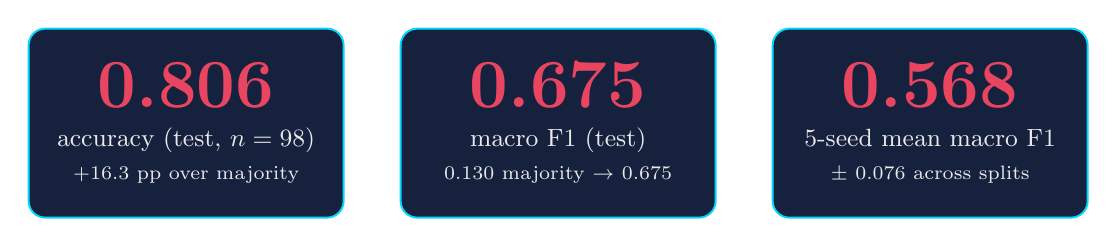
\begin{tikzpicture}[node distance=0.6cm and 0.7cm]
      \node[herostat] (acc) {%
        \textcolor{accent}{\Huge \textbf{0.806}}\\[0.2em]
        \small accuracy (test, $n=98$)\\
        \scriptsize +16.3 pp over majority
      };
      \node[herostat, right=of acc] (f1) {%
        \textcolor{accent}{\Huge \textbf{0.675}}\\[0.2em]
        \small macro F1 (test)\\
        \scriptsize 0.130 majority $\rightarrow$ 0.675
      };
      \node[herostat, right=of f1] (sweep) {%
        \textcolor{accent}{\Huge \textbf{0.568}}\\[0.2em]
        \small 5-seed mean macro F1\\
        \scriptsize $\pm$ 0.076 across splits
      };
    \end{tikzpicture}
  \end{center}

  \vspace{0.6em}
  \begin{center}
    \textcolor{accentblue}{Headline form is recoverable, structurally constrained, and stylistically decomposable.}
  \end{center}
\end{frame}

% ----------------------------------------------------------
% CORPUS FINDINGS
% ----------------------------------------------------------
\begin{frame}{Corpus-Level Findings}
  \begin{columns}
    \column{0.55\textwidth}
    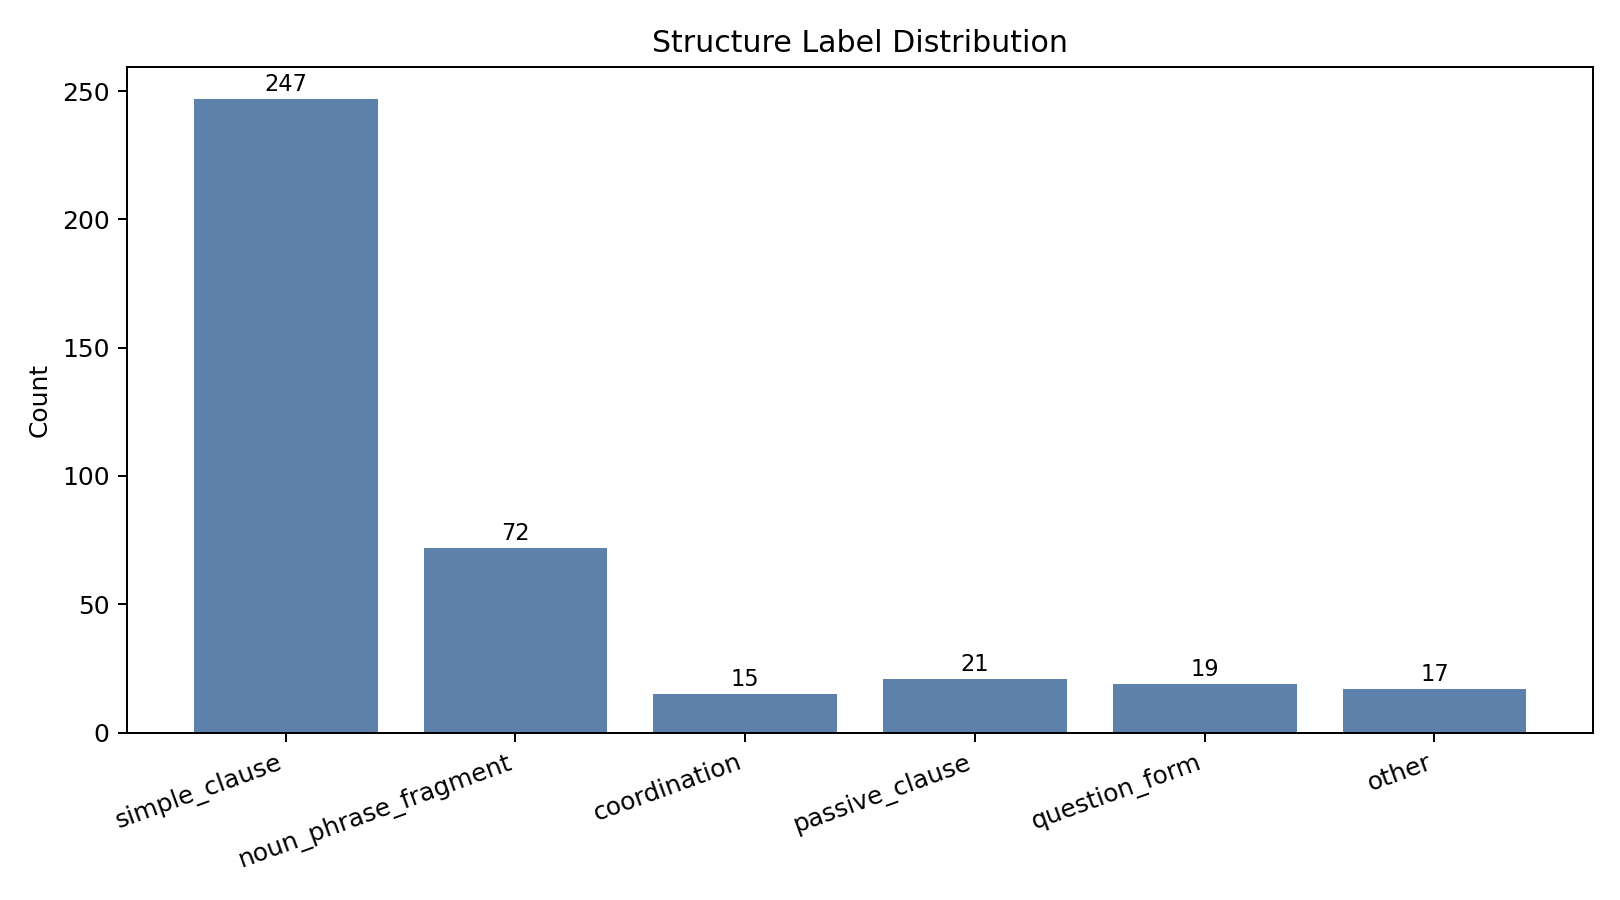
\includegraphics[width=\textwidth]{structure_label_distribution.png}

    \column{0.45\textwidth}
    \textbf{Headline profile}
    \begin{itemize}
      \item Avg length: 13.7 tokens
      \item Content-word ratio: 73.2\%
      \item Headlines with verbs: 92.1\%
      \item Active/non-passive: 94.6\%
      \item Named entities present: 95.7\%
      \item Actor/entity-first openings: 81.6\%
    \end{itemize}
  \end{columns}

  \vspace{0.5em}
  \textcolor{accent}{Finding: headline form is compact, entity-heavy, and strongly action-oriented.}
\end{frame}

% ----------------------------------------------------------
% PERFORMANCE SUMMARY
% ----------------------------------------------------------
\begin{frame}{Model Performance Overview}
  \begin{columns}
    \column{0.62\textwidth}
    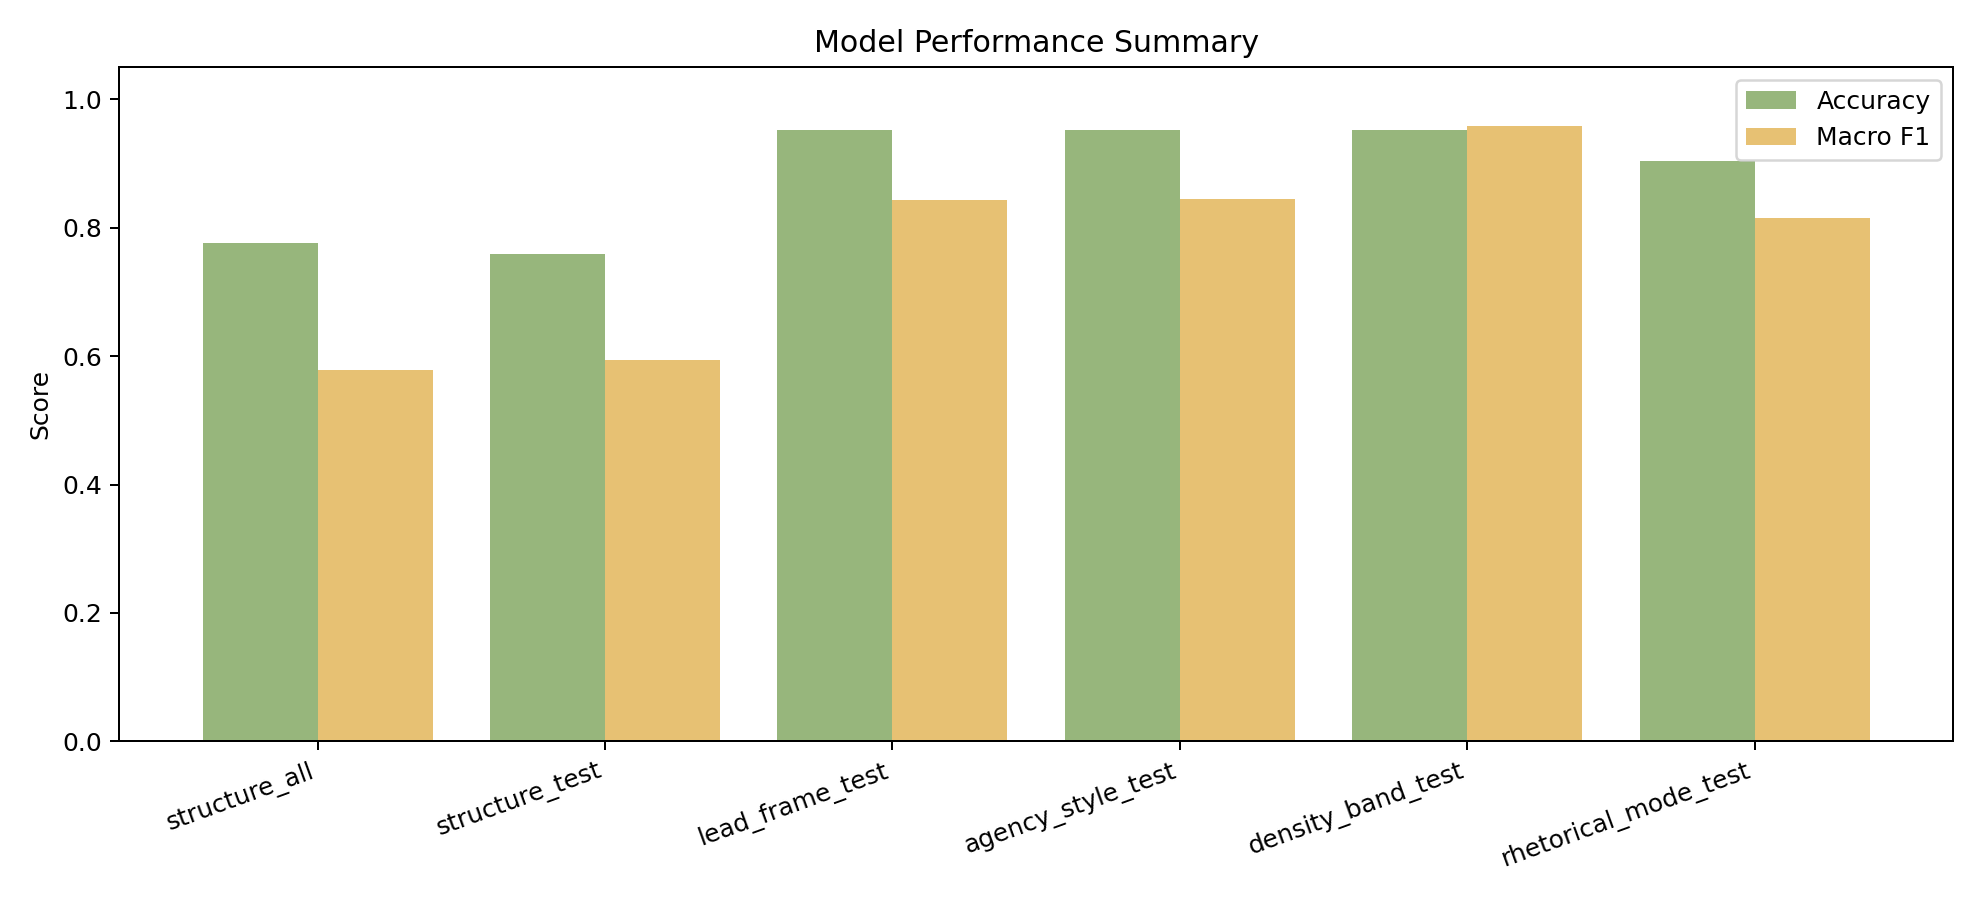
\includegraphics[width=\textwidth]{model_performance_summary.png}

    \column{0.38\textwidth}
    \small
    \textbf{Structure (held-out test)}
    \begin{itemize}
      \item Accuracy: \textcolor{accent}{0.806}
      \item Macro F1: \textcolor{accent}{0.675}
    \end{itemize}

    \textbf{Baselines (test)}
    \begin{itemize}
      \item Majority: 0.643 acc, 0.130 macro F1
      \item Random: 0.459 acc, 0.159 macro F1
    \end{itemize}

    \textcolor{accent}{+16.3 pp acc over majority; +34.7 pp over random.}
  \end{columns}
\end{frame}

% ----------------------------------------------------------
% STYLE SUMMARY
% ----------------------------------------------------------
\begin{frame}{Style Performance (held-out test)}
  \begin{center}
    \begin{tabular}{lcc}
      \toprule
      \textbf{Dimension} & \textbf{Accuracy} & \textbf{Macro F1} \\
      \midrule
      lead\_frame & 1.000 & 1.000 \\
      agency\_style & 0.908 & 0.428 \\
      density\_band & 1.000 & 1.000 \\
      rhetorical\_mode & 0.908 & 0.820 \\
      \bottomrule
    \end{tabular}
  \end{center}

  \vspace{1em}
  \begin{block}{Interpretation}
    Density and framing are highly recoverable; rhetorical mode remains harder because it depends on broader discourse cues and boundary judgments.
  \end{block}
\end{frame}

% ----------------------------------------------------------
% HEATMAP
% ----------------------------------------------------------
\begin{frame}{Performance Heatmap}
  \begin{center}
    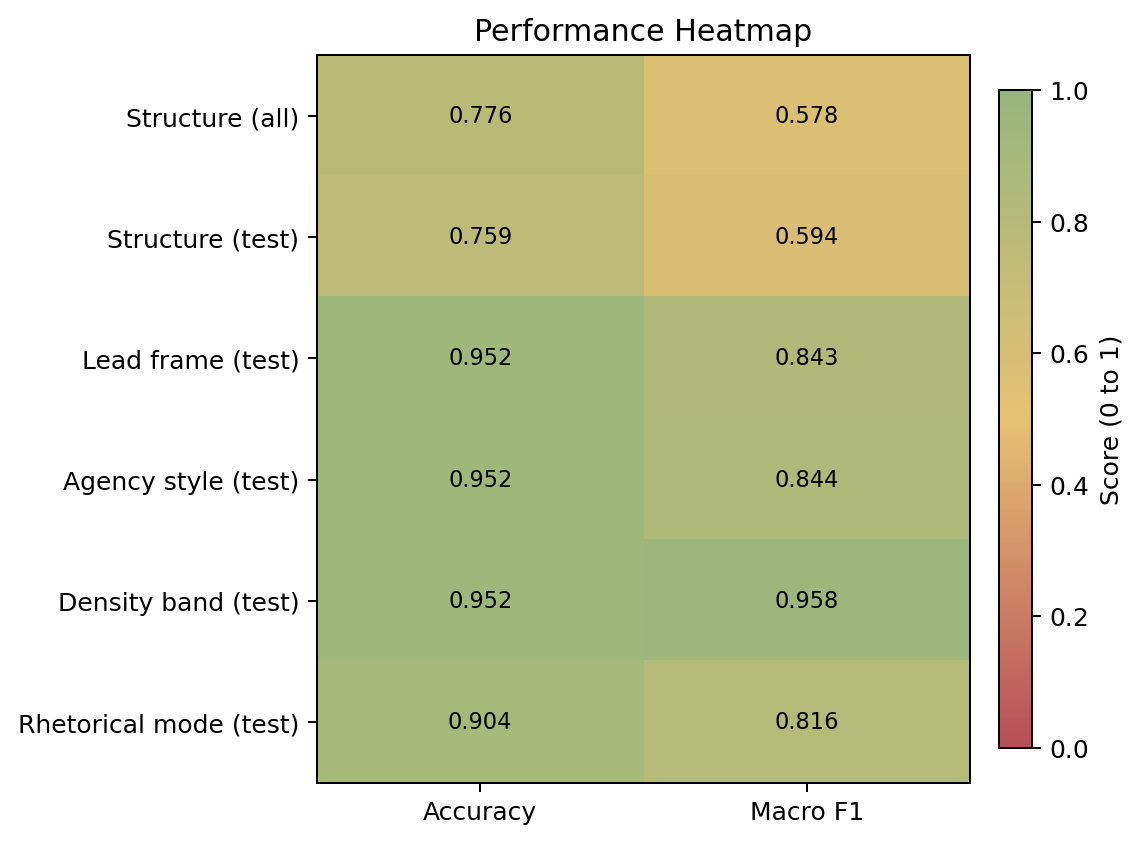
\includegraphics[height=0.78\textheight]{performance_heatmap.png}
  \end{center}
  \centering
  \textcolor{textsub}{Compact view of performance across structure and style outputs.}
\end{frame}

% ----------------------------------------------------------
% SEED STABILITY
% ----------------------------------------------------------
\begin{frame}{Seeding and Split Luck}
  \begin{columns}
    \column{0.62\textwidth}
    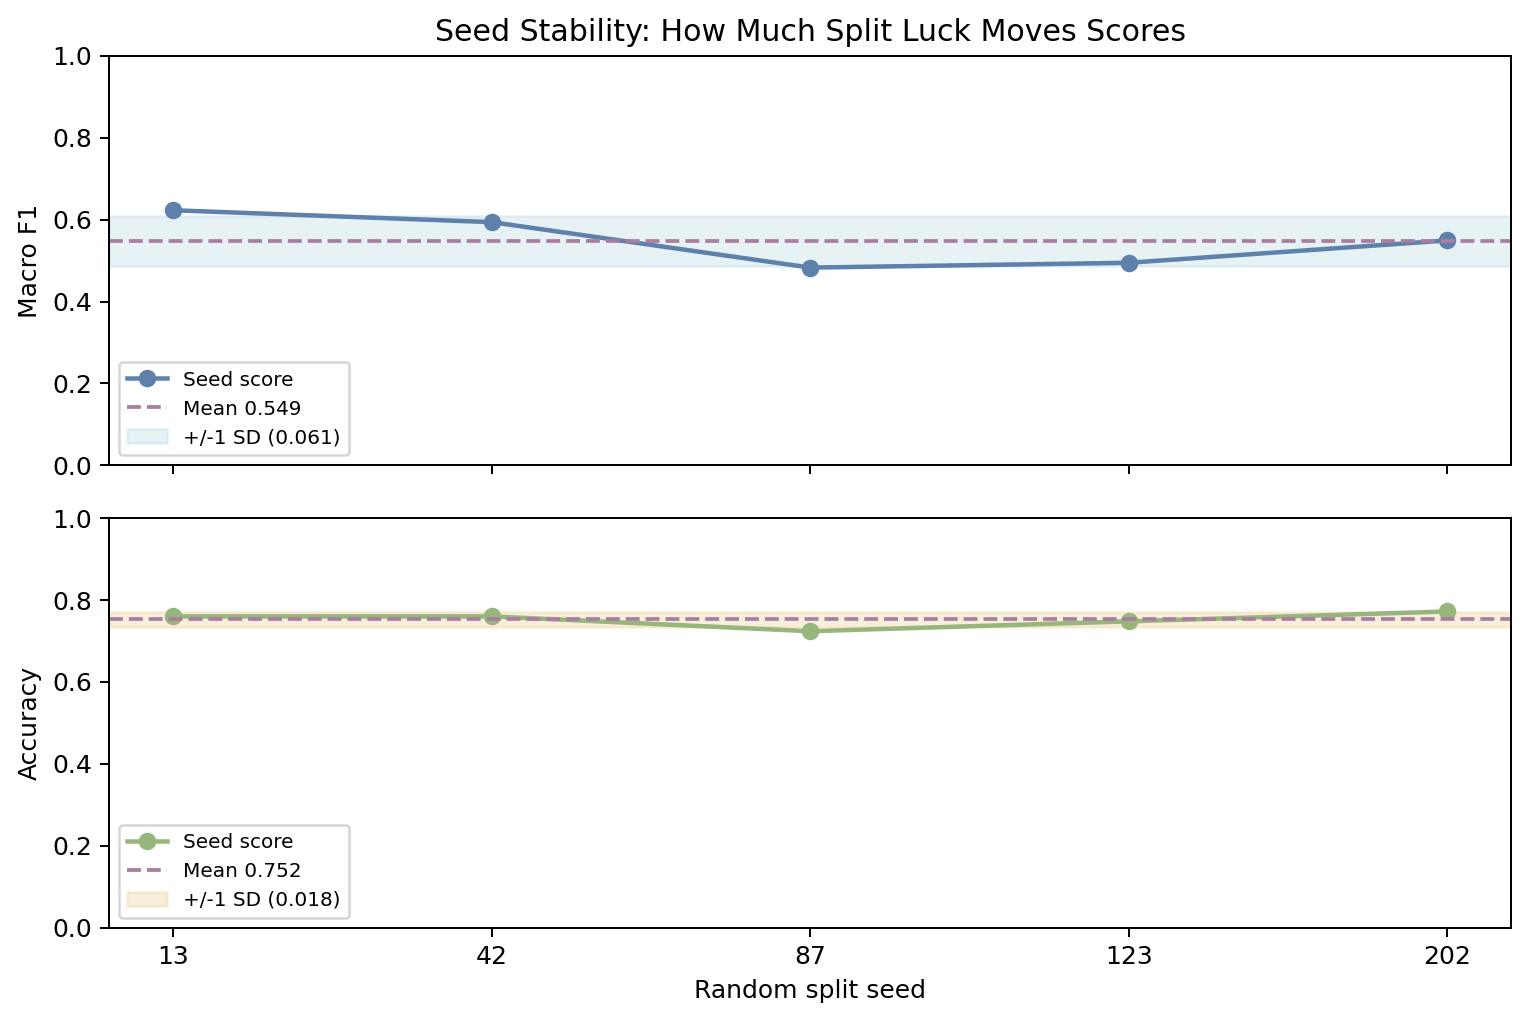
\includegraphics[width=\textwidth]{seed_stability_summary.png}

    \column{0.38\textwidth}
    \small
    \textbf{Why this analysis?}
    \begin{itemize}
      \item One split can be lucky/unlucky
      \item Need expected performance, not one draw
    \end{itemize}

    \textbf{5-seed summary}
    \begin{itemize}
      \item Test accuracy: $0.740 \pm 0.051$
      \item Test macro F1: $0.568 \pm 0.076$
      \item Dev macro F1: $0.608 \pm 0.073$
    \end{itemize}
  \end{columns}
\end{frame}

% ----------------------------------------------------------
% SEED INTERPRETATION
% ----------------------------------------------------------
\begin{frame}{Seeding and Split Luck (interpretation)}
  \begin{itemize}
    \item Per-seed structure test macro F1 spans \textbf{0.481 to 0.675} (spread 0.194).
    \item Per-seed structure test accuracy spans \textbf{0.663 to 0.806} (spread 0.143).
    \item Macro F1 varies more than accuracy, so class-balance behavior is the more split-sensitive quantity.
  \end{itemize}

  \vspace{0.8em}
  \begin{block}{Implication}
    Reporting only one split can overstate confidence. We therefore treat the seed mean as the expected score and the sample standard deviation as an uncertainty descriptor.
  \end{block}
\end{frame}

% ----------------------------------------------------------
% SPLIT STATS FORMULAS
% ----------------------------------------------------------
\begin{frame}{How We Quantify Split Variability}
  For metric values $m_1,\dots,m_K$ over $K$ random seeds:

  \[
  \bar{m} = \frac{1}{K}\sum_{i=1}^{K} m_i
  \]

  \[
  s = \sqrt{\frac{1}{K-1}\sum_{i=1}^{K}(m_i-\bar{m})^2}
  \]

  \vspace{0.8em}

  \begin{itemize}
    \item $\bar{m}$ estimates expected performance under split randomness
    \item $s$ measures split sensitivity (evaluation volatility)
    \item Per-seed trajectories reveal whether variance is smooth or driven by specific difficult splits
  \end{itemize}
\end{frame}

\section{Practical Use}

% ----------------------------------------------------------
% TUI
% ----------------------------------------------------------
\begin{frame}{Interactive TUI Sandbox for Journalists}
  \begin{columns}[T]
    \column{0.62\textwidth}
    \centering
    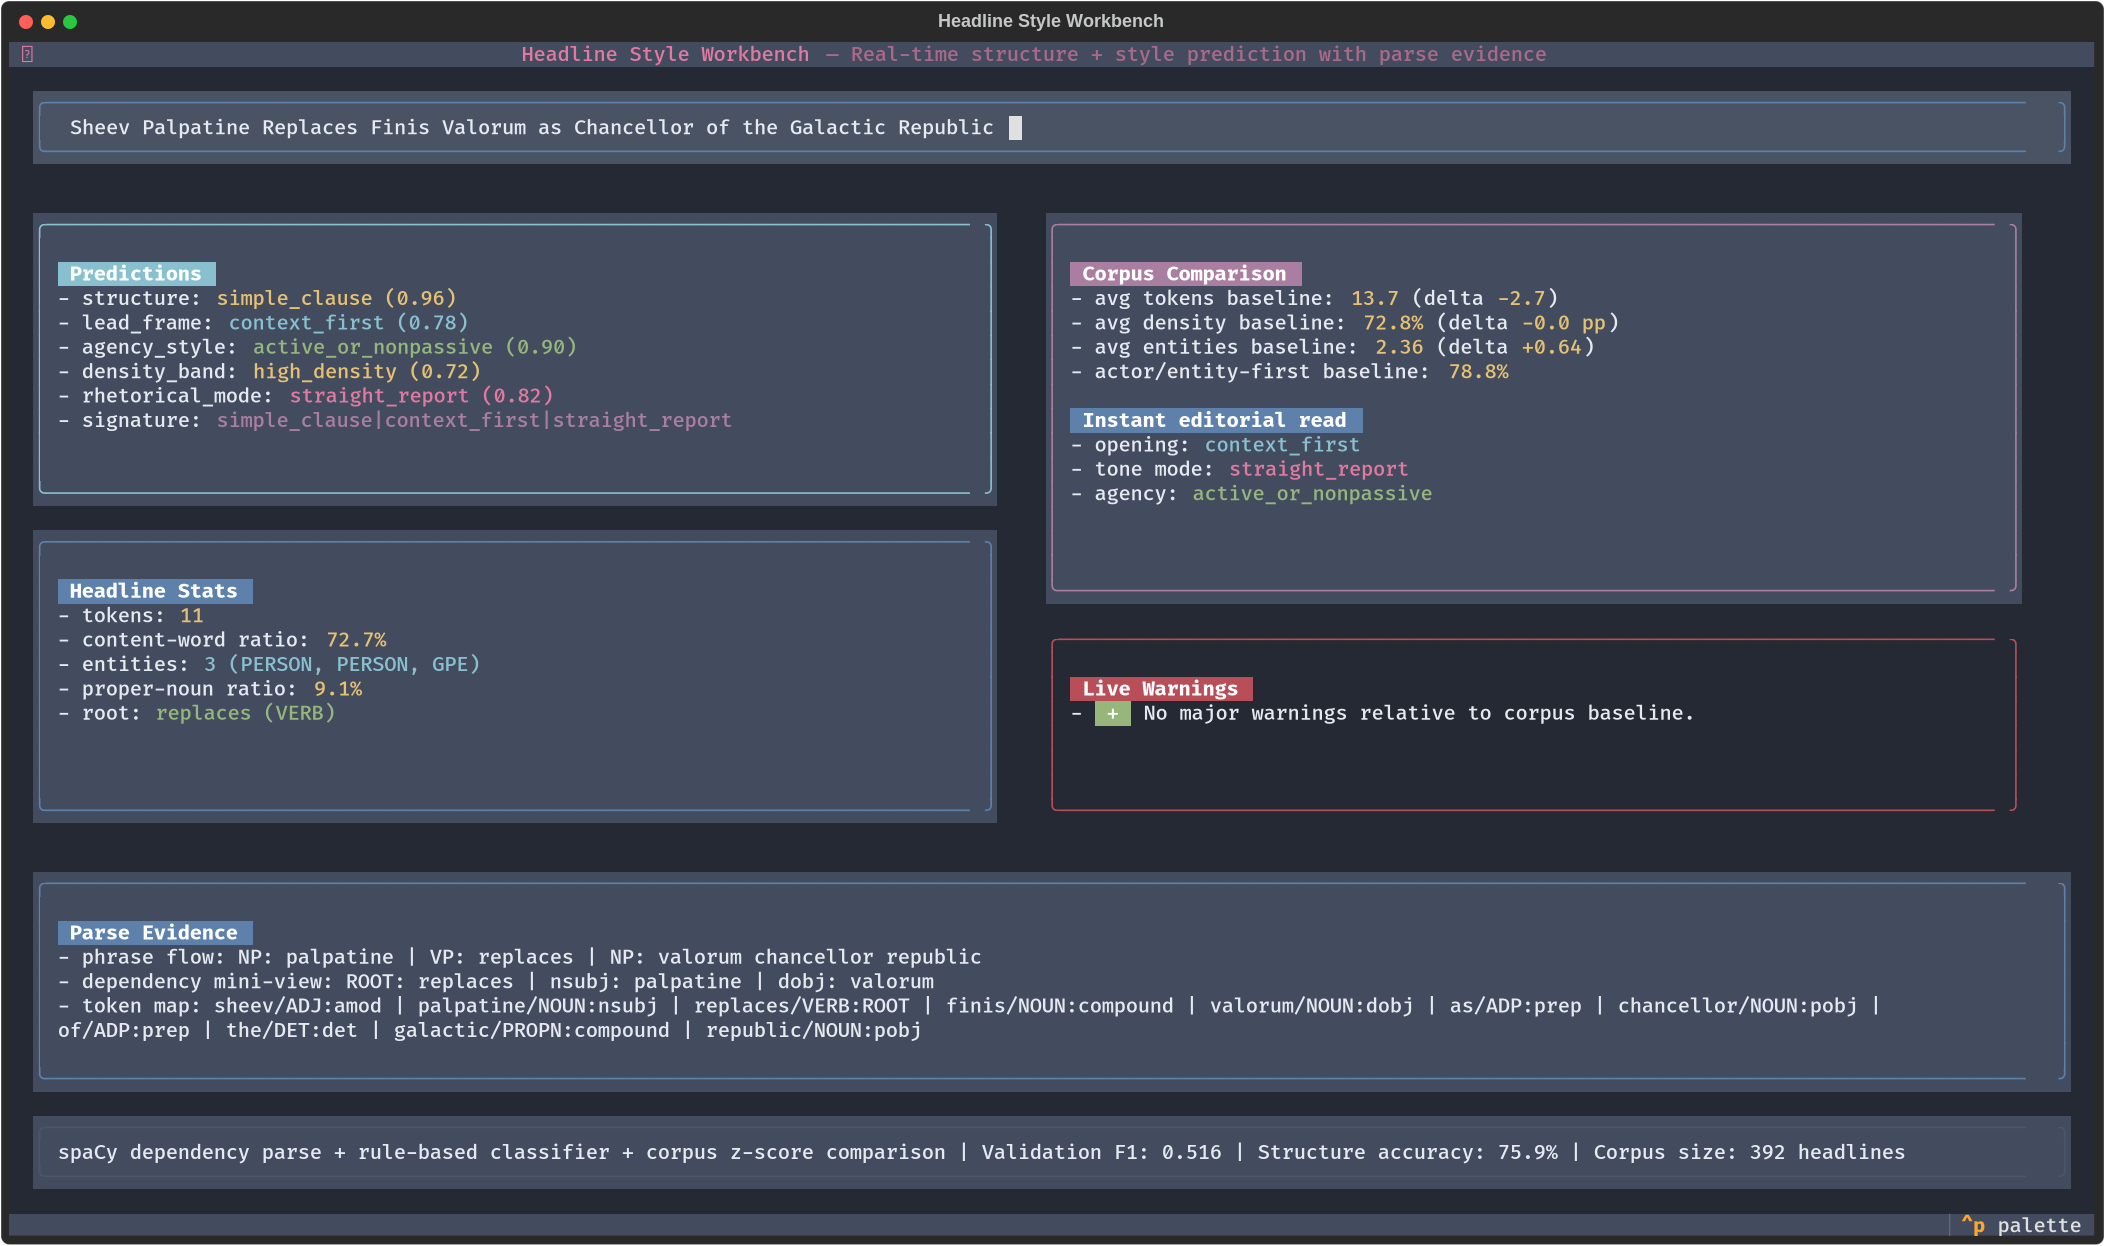
\includegraphics[width=\textwidth]{../images/tui_image.png}

    \column{0.38\textwidth}
    \small
    \textbf{What it enables}
    \begin{itemize}
      \item Real-time prediction + confidence
      \item Parse evidence per decision
      \item Instant headline A/B iteration
      \item Warnings for risky phrasing
    \end{itemize}

    \vspace{0.8em}
    \textcolor{accentblue}{A live sandbox for editorial A/B testing before publication.}
  \end{columns}
\end{frame}

\section{Wrap-up}

% ----------------------------------------------------------
% DISCUSSION
% ----------------------------------------------------------
\begin{frame}{Discussion: What Worked and What Remains Hard}
  \begin{columns}
    \column{0.5\textwidth}
    \textbf{Strong signals}
    \begin{itemize}
      \item Dominant templates are recoverable
      \item Multi-dimensional style profiling is informative
      \item Interpretability is operational, not cosmetic
    \end{itemize}

    \column{0.5\textwidth}
    \textbf{Difficult regions}
    \begin{itemize}
      \item Sparse ``other'' class behavior
      \item Coordination vs. simple-clause boundary cases
      \item Passive edge forms under punctuation/noise
    \end{itemize}
  \end{columns}

  \vspace{0.8em}
  \textcolor{accentblue}{Interpretation: gains are large versus baseline, but minority-structure distinctions remain the principal error source.}
\end{frame}

% ----------------------------------------------------------
% LIMITATIONS
% ----------------------------------------------------------
\begin{frame}{Limitations}
  \begin{itemize}
    \item Rule-based systems are highly interpretable but less flexible than fully learned models
    \item Class imbalance can mask minority-class weaknesses
    \item Some labels remain intrinsically subjective at boundary cases
    \item Source and language scope limit broad external generalization
    \item No external lexical expansion in this phase (intentional scope constraint)
  \end{itemize}

  \vspace{1em}
  \textcolor{accent}{Despite these limits, structural signal remains strong and measurable.}
\end{frame}

% ----------------------------------------------------------
% CONCLUSION
% ----------------------------------------------------------
\begin{frame}{Conclusion}
  \begin{center}
    \Large
    \textcolor{accent}{\textbf{Headlines are structured linguistic products}}\\[0.4em]
    \large not free-form snippets\\[1.0em]

    \textcolor{accentblue}{\textbf{Structure test: 0.806 accuracy, 0.675 macro F1}}\\[0.4em]
    \textcolor{textsub}{with explicit split-luck quantification}
  \end{center}

  \vspace{1.4em}

  \begin{block}{Bottom Line}
    Interpretable NLP can capture headline form, evaluate it against human gold standards, and provide practical editorial tooling through a real-time sandbox interface.
  \end{block}
\end{frame}

\begin{frame}[plain]
  \begin{center}
    \vspace{2.5em}
    \Huge
    \textit{``Headline form is measurable,}\\[0.3em]
    \textit{predictable, and actionable.''}

    \vspace{2.5em}
    \normalsize
    \textcolor{textsub}{Victor Derani \quad$\cdot$\quad Avi Herman \quad$\cdot$\quad Kylie Lin}\\[0.3em]
    \textcolor{textsub}{\small github.com/avih7531/headline-structure-analysis}
  \end{center}
\end{frame}

\end{document}

